

\tikzset{every picture/.style={line width=0.75pt}} %set default line width to 0.75pt        

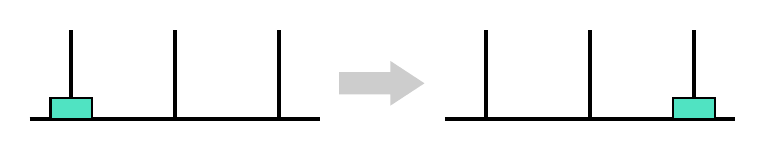
\begin{tikzpicture}[x=0.75pt,y=0.75pt,yscale=-1,xscale=1]
%uncomment if require: \path (0,387); %set diagram left start at 0, and has height of 387

%Straight Lines [id:da40902814921476005] 
\draw [line width=1.5]    (0,43) -- (140,43) ;
%Straight Lines [id:da32687008830530373] 
\draw [line width=1.5]    (20,43) -- (20,0) ;
%Straight Lines [id:da3172525661879657] 
\draw [line width=1.5]    (70,43) -- (70,0) ;
%Straight Lines [id:da3724427659815115] 
\draw [line width=1.5]    (120,43) -- (120,0) ;
%Shape: Rectangle [id:dp12926306550885913] 
\draw  [fill={rgb, 255:red, 80; green, 227; blue, 194 }  ,fill opacity=1 ] (10,33) -- (30,33) -- (30,43) -- (10,43) -- cycle ;
%Straight Lines [id:da944371051878028] 
\draw [line width=1.5]    (200,43) -- (340,43) ;
%Straight Lines [id:da5623860802403418] 
\draw [line width=1.5]    (220,43) -- (220,0) ;
%Straight Lines [id:da9847294698370319] 
\draw [line width=1.5]    (270,43) -- (270,0) ;
%Straight Lines [id:da7330741622812829] 
\draw [line width=1.5]    (320,43) -- (320,0) ;
%Shape: Rectangle [id:dp6766108174560563] 
\draw  [fill={rgb, 255:red, 80; green, 227; blue, 194 }  ,fill opacity=1 ] (310,33) -- (330,33) -- (330,43) -- (310,43) -- cycle ;
%Right Arrow [id:dp9017051385213559] 
\draw  [draw opacity=0][fill={rgb, 255:red, 155; green, 155; blue, 155 }  ,fill opacity=0.5 ] (149,20.4) -- (173.71,20.4) -- (173.71,15) -- (190.18,25.8) -- (173.71,36.59) -- (173.71,31.19) -- (149,31.19) -- cycle ;




\end{tikzpicture}